% ### Uses XeLaTeX ### %
% ### Needs beamer-master ### %
\documentclass[aspectratio=169]{beamer} %. Aspect Ratio 16:9
\usetheme{AI2} % beamerthemeSprace.sty
% DATA FOR FOOTER
\date{2019}
\title{}
\author{}
\institute{Advanced Institute for Artificial Intelligence (AI2)}
\begin{document}    
% ####################################
% FIRST SLIDE 						:: \SliTit{<Title of the Talk>}{<Author Name>}{<Intitution>}
% SLIDE SUB-TITLE					:: \SliSubTit{<Title of the Chapter>}{<Title of the Section>}
% SLIDE WITH TITLE 					:: \SliT{<Title>}{Content}
% SLIDE NO TITLE 						:: \Sli{<Content>} 
% SLIDE DOUBLE COLUMN WITH TITLE 	:: \SliDT{<Title>}{<First Column>}{<Second Column>}
% SLIDE DOUBLE COLUMN NO TITLE 		:: \SliD{<First Column>}{<Second Column>}
% SLIDE ADVANCED WITH TITLE 			:: \SliAdvT{<Title>}{<Content>}
% SLIDE ADVANCED  NO TITLE 			:: \SliAdv{<Content>}
% SLIDE ADVANCED DOUBLE TITLE 		:: SliAdvDT{<Title>}{<First Column>}{<Second Column>}
% SLIDE ADVANCED DOUBLE NO TITLE 	:: SliAdvD{<First Column>}{<Second Column>}
% ITEMIZE 							:: \begin{itemize}  \IteOne{1st Level} \IteTwo {2nd Level} \IteThr{3rd Level} \end{itemize}
% SECTION 							:: \secx{Section} | \secxx{Sub-Section}
% COLOR BOX 						:: \blu{blue} + \red{red} + \yel{yellow} + \gre{green}
% FRAME 							:: \fra{sprace} \frab{blue} \frar{red} + \fray{yellow} + \frag{green}	
% REFERENCE						:: \refer{<doi number>}
% FIGURE 							::  \img{X}{Y}{<scale>}{Figures/.png} 
% FIGURE							:: \begin{center}\includegraphics[scale=<#>]{Figures/.png}\end{center}
% PROJECT STATUS					:: \planned\~    \started\~   \underway\~   \done\~   
% EXERCICIO							:: \Exe{<#>}{<text>}
% STACKREL							:: \underset{<down>}{<up>}
% FLUSH LEFT						:: \begin{flalign*}  & <1st equation> & \\  & <12nd equation>  & \\ \end{flalign*}
% REAL / IMAGINAY					:: \Re / \Im
% SLASH								:: \sl{} or \sl
% BOLD MATH							:: \pmb{<>}
% ####################################
%
% FIRST SLIDE :: DO NOT BREAK LINE !!!
\SliTit{Introdução a Estatística}{Advanced Institute for Artificial Intelligence}{https://advancedinstitute.ai}

% SLIDE WITH TITLE
\SliT{Sumário}{

\begin{itemize}
  \IteOne{Introdução}
  \IteOne{Módulos}
  \IteOne{Exemplos}
\end{itemize}

}

% SLIDE WITH TITLE
\SliT{Introdução a Estatística}{

Estatística

\begin{itemize}
  \IteOne{Ciência de aprendizagem a partir de dados.}
  \IteOne{Métodos que auxiliam o processo de tomada de decisão.}
\IteOne{A Estatística está presente em todas as áreas da ciência que envolvam a coleta e análise de dados.}

\end{itemize}
}

\SliT{Introdução a Estatística}{

\begin{itemize}
  \IteOne{Dados:}
  \IteTwo{Observações de uma ou mais variáveis.}
  \IteTwo{Variável é aquilo que se deseja observar para obter algum conhecimento, por ex., idade, sexo, peso e outras.}
\end{itemize}
}
% SLIDE WITH TITLE
\SliT{Introdução a Estatística}{

\begin{itemize}
  \IteOne{Estatística: envolve coletar, classificar, resumir, organizar, analisar e interpretar dados.}
  \IteOne{Envolve:}
  \IteTwo{Descrever Conjuntos de Dados}
  \IteTwo{Tirar conclusões (fazer estimativas, decisões, previsões, etc. a cerca de conjuntos de dados}
\end{itemize}

}

\SliT{Introdução a Estatística}{

\begin{itemize}
  \IteOne{Estatística descritiva: descrever os dados}
  \IteTwo{Coletar, Apresentar e caracterizar}
  \IteOne{Estatística inferencial: tomar decisão baseado nas características da população}
  \IteTwo{Estimativa, teste de hipótese}
  
\end{itemize}


}

\SliT{Introdução a Estatística}{

\begin{itemize}
  \IteOne{ Unidade experimental: objeto sobre o qual coletamos dados}
\IteOne{ População: todos os itens de interesse}
\IteOne{ Variável: um conjunto de valores registrados para uma unidade experimental individual}
\IteOne{ Amostra: subconjunto de uma população}
\end{itemize}

}

\SliT{Introdução a Estatística}{

\begin{itemize}
  \IteOne{Inferência estatística: estimativa ou previsão ou generalização sobre uma população com base nas informações contidas em uma amostra}
\IteOne{Medida de Confiabilidade: declaração (geralmente qualificada) sobre o grau de incerteza associado a uma inferência estatística}
\end{itemize}

}

\SliT{Introdução a Estatística}{

\begin{itemize}
  \IteOne{As variáveis podem ser categóricas (qualitativas) ou
numéricas (quantitativas)}
\IteTwo{Variáveis qualitativas: São características de uma
população que não pode ser medidas.}
\IteTwo{Ordinais: Grau de gravidade de uma doença}
\IteTwo{Nominais: Presença de um sintoma}
\IteTwo{Variáveis quantitativas: São características de uma população que pode ser quantificadas.}
\IteTwo{Discretas: Número de cirurgias}
\IteTwo{Contínuas: Idade, Pressão Arterial}
\end{itemize}

}

\SliT{Introdução a Estatística}{

Obtendo dados para análises estatísticas:

\begin{itemize}
  \IteOne{Fonte publicada: livro, jornal, jornal, site}
  \IteOne{Experiência projetada: pesquisador exerce controle rígido sobre as unidades}
  \IteOne{Pesquisa: um grupo de pessoas é pesquisado e suas respostas são registradas}
  \IteOne{Estudo de observação: unidades são observadas em ambiente natural e variáveis de interesse são registradas}
\end{itemize}

}

\SliT{Introdução a Estatística}{

\begin{itemize}
  \IteOne{Estatística é uma técnica essencial para responder questões científicas}
  \IteOne{Para isso são realizados estudos experimentais ou observacionais}
  \IteOne{O padrão de variação nos dados faz com que
a resposta não seja óbvia}

\end{itemize}

}

\SliT{Introdução a Estatística}{

Amostragem dos dados:

\begin{itemize}
  \IteOne{A amostra deve ser representativa do problema em estudo}
  \IteOne{O tamanho da amostra deve ser suficiente para representar o problema}
  \IteOne{Aleatoriedade da amostra: garantir que todos os elementos da população tenham chance de pertencer à amostra}
\end{itemize}

}

\SliT{Introdução a Estatística}{

Epíciclos de ciência dos dados \footnote{"The Art of Data Science A Guide for Anyone Who Works with Data". Roger D. Peng and Elizabeth Matsui. 2016}

\begin{center}
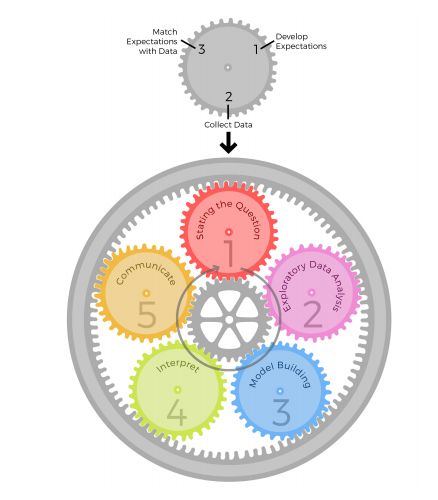
\includegraphics[scale=0.32]{epi.png}     
\end{center}

}

\SliT{Introdução a Estatística}{

\begin{itemize}
\IteOne{ Os epíciclos de ciência dos dados são etapas genéricas que podem ter complexidade variável}
\IteOne{ Um projeto pode ser feito seguindo cada etapa em apenas um dia }
\IteOne{ Projetos maiores podem demandar a execução de cada etapa por dias ou meses}
\end{itemize}

}

\SliT{Introdução a Estatística}{

Etapas dp epicíclo:

\begin{itemize}
\IteOne{ Definir a questão}
\IteOne{ Análise de Dados Exploratória}
\IteOne{ Construção de um modelo}
\IteOne{ Interpretação}
\IteOne{ Comunicação}
\end{itemize}

}

\SliT{Introdução a Estatística}{

Cada etapa segue um processo de alinhamento de expectativa

\begin{itemize}
\IteOne{ Estabelecendo Expectativas }
\IteOne{ Coletando informações (dados), comparando os dados com
suas expectativas e, se as expectativas não corresponderem,}
\IteOne{ Revise suas expectativas ou ajuste os dados para que seu dados e suas expectativas correspondam.}
\end{itemize}

}
\SliT{Introdução a Estatística}{

Forma de representação da freqüência de cada valor distinto da variável em estudo. 

Juntamente com as freqüências simples, a tabela
poderá ainda incluir:

\begin{itemize}
\IteOne{Frequências relativas:  percentagem relativa à freqüência}
\IteOne{Frequências acumuladas: número de vezes que uma
variável assume um valor inferior ou igual a esse valor. }
\IteOne{Frequências relativas acumuladas: percentagem
relativa à freqüência acumulada }
\end{itemize}

}

\SliT{Introdução a Estatística}{

Listagem de modo de contração por colaborador

\begin{center}
\begin{tabular}{ c c }
Nome	& Modo de contratação \\
Bernita Lawhon &	CLT \\
Caron Abernathy &	PJ \\
Rita Figgins &	PJ \\
Bulah Zackery &	PJ \\
Ja Berber &	CLT \\
Tennille Verrill &	CLT \\
Francina Samaniego &	PJ \\
Elinor Sowder &	PJ \\
Shantay Crane &	CLT \\
Suzan Coldwell &	PJ 
\end{tabular}
\end{center}

}

\SliT{Introdução a Estatística}{

Tabela de frequência de contagem de tipo de contração

\begin{center}
\begin{tabular}{ c c c}
Modo de contratação & Frequência absoluta & frequência relativa  \\
PJ	&  	6 & 6 -$>$ 10 60\% \\
CLT	&  	4 & 6 -$>$ 10 40\% \\	
Total	&  	10 & 100\% 	
\end{tabular}
\end{center}

}
\SliT{Introdução a Estatística}{

Elementos essenciais  uma tabela
\begin{itemize}
\IteOne{Título: uma indicação que antecede a tabela e explique tudo referente a tabela.}
\IteOne{Cabeçalho: colocado na parte superior da tabela, especificando o conteúdo das colunas.}
\IteOne{Corpo: corresponde ao conjunto de colunas e de linhas que contêm informações sobre o fenômeno estudado.}
\end{itemize}
}

\SliT{Introdução a Estatística}{

Recomendações quando a construção de gráficos

\begin{itemize}
\IteOne{Todo gráfico deve ter título, escala e fonte de
dados}
\IteOne{As escalas devem crescer da esquerda para a direita e de baixo para cima.}
\IteOne{As distâncias que indicam as unidades devem ser  uniformes.}
\end{itemize}

}

\SliT{Introdução a Estatística}{

Sumarização de variável qualitativa:
\begin{itemize}
\IteOne{Tabelas usando contagens ou porcentagens}
\IteOne{Gráfico de Barras ou Gráfico de Setores}
\end{itemize}

}

\SliT{Introdução a Estatística}{
\begin{center}
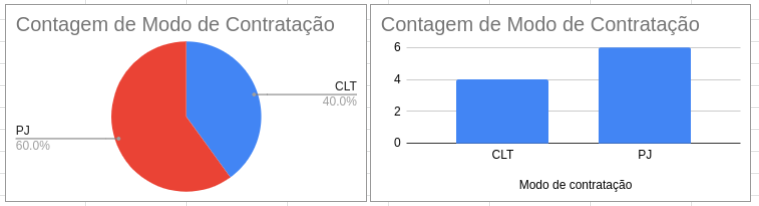
\includegraphics[scale=0.55]{1111.png}     
\end{center}
}
\SliT{Introdução a Estatística}{

Tabela de variáveis quantitativas - Nível de consumo de alcool.

\begin{center}
\begin{tabular}{ c c}
\textbf{local}	& \textbf{nível} \\
Belarus	& 17.5 \\
Moldova	& 16.8 \\
Lithuania &	15.4 \\
Russia	& 15.1 \\
Romania	& 14.4 \\
Ukraine	& 13.9 \\
Andorra	& 13.8 \\
Hungary	& 13.3 \\
Czech Republic	& 13.0 \\
Slovakia &	13.0 \\
\end{tabular}
\end{center}

}

\SliT{Introdução a Estatística}{

Sumarização de variável quantitativas:
\begin{itemize}
\IteOne{Tabelas de Freqüências}
\IteOne{Histograma}
\end{itemize}

}

\SliT{Introdução a Estatística}{

Critério para determinar a quantidade de classes:

\[ k = 1+3.3+log(n) \]

Amplitude das classes

\[ a = (maiorValor-menorValor/numeroDeClasses) \]

no pandas a quantidade de classes é definida por série usando o parâmetro bins do método value_counts()


}

\SliT{Introdução a Estatística}{

Histograma: Representação gráfica da distribuição das frequências absolutas ou relativas Normalmente utilizado para variáveis contínuas.

\begin{itemize}
\IteOne{ As barras devem estar todas juntas }
\IteOne{ Cada barra representa a freqüência de um intervalo de valores }
\IteOne{ Os intervalos devem ter todos a mesma amplitude }
\end{itemize}

}

\SliT{Introdução a Estatística}{

Medidas de Tendência Central:

\begin{itemize}
\IteOne{Servem para termos uma idéia acerca dos valores médios da variável em estudo}
\IteOne{São usados para sintetizar em um único número os dados observados}
\IteOne{São exemplos de medidas de tendência central: Média, Moda e Mediana}
\end{itemize}

}

\SliT{Introdução a Estatística}{
Medidas Separatrizes separam a distribuição em partes iguais (depois de ordenadas). 

\begin{itemize}
\IteOne{ Quartis (quatro partes)}
\IteOne{ Decis (dez partes)}
\IteOne{ Percentis (cem partes)}
\end{itemize}

}

 \SliT{Introdução a Estatística}{
\begin{center}
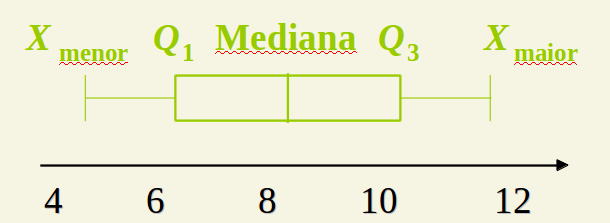
\includegraphics[scale=0.70]{1212.png}     
\end{center}
}

\SliT{Introdução a Estatística}{
Gráficos do tipo boxplot representam gráficamente cinco medidas separatrizes: 

\begin{itemize}
\IteOne{ mínimo}
\IteOne{ quartil inferior}
\IteOne{ mediana}
\IteOne{ quartil superior}
\IteOne{ máximo}
\end{itemize}

Esse gráfico é útil para identificar valores chamados \textit{outliers}, que são valores muito altos ou muito baixos em relação ao restante da população

}



\SliT{Introdução a Estatística}{
\begin{itemize}
\IteOne{ Medidas de Variabilidade reflitem a variação dentro de um conjunto de dados}
\IteOne{ Essas medidas serão pequenas se os dados forem próximos e grandes se eles estiverem muito espalhados.}
\IteOne{ permitem comparar amostras de diferentes tamanhos e determinar se uma amostra é mais variável (ou heterogênea) que outra.}
\end{itemize}

}

\SliT{Introdução a Estatística}{

\begin{itemize}
\IteOne{ Variância: é um indicativo da dispersão de um conjunto de dados em relação à média }
\IteOne{ Desvio Padrão: Corresponde à raiz quadrada da variância }
\IteOne{ A medida mais usada na comparação de diferenças entre grupos }
\IteOne{ Quanto maior o desvio-padrão, maior a variabilidade
dos dados}

\end{itemize}
}

% \SliT{Introdução a Estatística}{

% Análise Bivariada

% \begin{itemize}
% \IteOne{ Investigar relação entre variáveis categóricas}
% \IteOne{ Podemos construir tabelas de freqüência com dupla entrada. Essas tabelas de dados cruzados são conhecidas por tabelas de contingência  }
% \end{itemize}

% }

% \SliT{Introdução a Estatística}{

% Box-Plot - deixar para mostrar depois!!
% Representação gráfica de cinco medidas: mínimo,
% quartil inferior, mediana, quartil superior, máximo
% }

% \SliT{Introdução a Estatística}{

% Exemplo de tabela de frequências
% }

% \SliT{Introdução a Estatística}{

% Exemplo de tabela de frequências
% }
% \SliT{Introdução a Estatística}{

% \begin{itemize}
%   \IteOne{Dados quantitativos são medições registradas em uma escala numérica que ocorre naturalmente.}
%   \IteTwo{Medido em escala numérica: número de itens com defeito em um lote.}
%   \IteOne{Dados qualitativos são medições que não podem ser medidas em uma escala numérica natural; eles só podem ser classificados em um de um grupo de categorias.}
%   \IteTwo{Classificado em categorias: gênero de empregados de uma empresa}
% \end{itemize}

% }

% \SliT{Introdução a Estatística}{

% \begin{itemize}
%   \IteOne{Uma amostra representativa exibe características típicas presentes na população de interesse.}
%   \IteOne{Uma amostra aleatória simples de n unidades experimentais é uma amostra selecionada da população de tal maneira que cada amostra diferente de tamanho n tem uma chance igual de seleção.}
% \end{itemize}

% }


% \SliT{Introdução a Estatística}{
% %\begin{center}
% %\includegraphics[scale=0.27]{vv.png}     
% %\end{center}
% }

\end{document}